
\pdfbookmark{Основное содержание работы}{content}
\section*{Основное содержание работы}

\pdfbookmark[1]{Введение}{introduction}

\highlight{Во введении} обоснована актуальность темы исследования, показана степень ее разработанности, сформулированы цель и задачи работы, приведены научная новизна, теоретическая и практическая значимость, а также положения, выносимые на защиту.

\pdfbookmark[1]{Глава 1. Проблемы создания расчетных динамических моделей конструкций по результатам модальных испытаний}{partReview}

\highlight{В первой главе} выполнен обзор методов коррекции и ассемблирования расчетных моделей. Приведены основные теоретические сведения о методах классического и операционного модального анализа. Показано, что известные методы коррекции не всегда могут быть использованы для коррекции расчетных моделей летательных аппаратов, а во многих случаях не позволяют получить достоверные результаты.

\pdfbookmark[1]{Глава 2. Коррекция и синтез расчетных динамических моделей конструкций}{partModelUpdating}

\highlight{Вторая глава} посвящена разработке и развитию методик коррекции, освобождения и синтеза расчетных динамических моделей по результатам модальных испытаний. Математическая постановка задачи коррекции допускает изменение как упругих, так и диссипативных характеристик расчетной модели. Методика коррекции основывается на дополнении исходной конечно-элементной модели внутренними и внешними корректирующими элементами. Первые определяют изменение характеристик самой модели, а вторые ответственны за коррекцию параметров внешних связей, накладываемых на модель. Корректирующие элементы строятся на узлах исходной модели. 

Рассматривается конечно-элементная модель исследуемого объекта в виде матриц жесткости $ \mat{K} $ и масс $ \mat{M} $. Собственные числа $ \lambda = 2 \pi \nu $ (где $ \nu $~---~частота собственных колебаний) и формы колебаний $ \mat{Y} $ определяются из решения обобщённой проблемы собственных значений:
\begin{equation}
	\rbrackets{\mat{K} - \lambda \mat{M}} \mat{Y} = 0.
\end{equation}

Обладая конструкторской документацией и результатами взвешивания конструкции, инерционные характеристики модели могут быть определены достаточно точно. Однако уточнение упругих характеристик модели не столь однозначно в силу совокупного объема факторов, обуславливающих погрешности моделирования: дискретизация модели, неточность задания упругих свойств материалов и граничных условий. Поэтому, полагая матрицу масс определенной точно, изменения вносятся только в матрицу жесткости путем добавления к исходной матрице $ \mat{K} $ матрицы жесткости корректирующей КЭ-модели $ \Delta \mat{K} $. При этом корректирующая матрица жесткости записывается в виде:
\begin{equation}
	\Delta \mat{K} = \Delta \internal{\mat{K}} + \Delta \external{\mat{K}}, \label{eq:stiffMatrixDecomposition}
\end{equation}
где $ \Delta \internal{\mat{K}} $ и $ \Delta \external{\mat{K}} $~---~матрицы жесткости внутренних и внешних корректирующих элементов.

Матрица жесткости внутреннего корректирующего элемента в общем случае имеет вид:
\begin{equation}
	\Delta \internal{\mat{K}}_j = \sum\limits_{p\,=\,1}^{q} \internal{c}_{j+p-1} \mat{G}_j^{(p)}, \ j = 1 \hdots e,
\end{equation}
где $ \internal{c}_{j+p-1} $~---~неизвестная внутренняя корректирующая жесткость; $ q $~---~число внутренних корректирующих жесткостей, описывающих элемент; $ \mat{G}_j^{(p)} $~---~парциальная матрица жесткости внутреннего коррректирующего элемента; $ e $~---~число внутренних корректирующих элементов. 

Число корректирующих жесткостей $ q $ зависит от числа физических параметров, которыми описывается добавляемый элемент. В случае, если динамические свойства модели существенно зависят от изгибных и крутильных жесткостей её балочных или оболочечных элементов, предлагается использовать корректирующую КЭ-модель из балочных элементов ($ q = 4 $). В этом случае парциальные матрицы корректирующего элемента примут вид:
\begin{equation*}
	\begin{gathered}
	\mat{G}_j^{(1)} =
	\begin{pmatrix}
		\mat{D}_1 & \mat{0} & -\mat{D}_1 & \mat{0} \\
		\mat{0} & \mat{0} & \mat{0} & \mat{0} \\
		-\mat{D}_1 & \mat{0} & \mat{D}_1 & \mat{0} \\
		\mat{0} & \mat{0} & \mat{0} & \mat{0} \\
	\end{pmatrix},
	\mat{G}_j^{(2)} =
	\begin{pmatrix}
		6 \mat{D}_2 & 3 \ell \mat{D}_4 & -6 \mat{D}_2 & 3 \ell \mat{D}_4 \\
		3 \ell \trans{\mat{D}}_4 & 2 \ell ^ 2 \mat{D}_3 & -3 \ell \trans{\mat{D}}_4 & \ell ^ 2 \mat{D}_3 \\
		-6 \trans{\mat{D}}_2 & -3 \ell \mat{D}_4 & 6 \mat{D}_2 & -3 \ell \mat{D}_4 \\
		3 \ell \trans{\mat{D}}_4 & \ell ^ 2 \trans{\mat{D}}_3 & -3 \ell \trans{\mat{D}}_4 & 2 \ell ^ 2 \mat{D}_3
	\end{pmatrix}, \\
	\mat{G}_j^{(3)} =
	\begin{pmatrix}
		6 \mat{D}_3 & -3 \ell \trans{\mat{D}}_4 & -6 \mat{D}_3 & -3 \ell \trans{\mat{D}}_4 \\
		-3 \ell \mat{D}_4 & 2 \ell ^ 2 \mat{D}_2 & 3 \ell \mat{D}_4 & \ell ^ 2 \mat{D}_2 \\
		-6 \trans{\mat{D}}_3 & 3 \ell \trans{\mat{D}}_4 & 6 \mat{D}_3 & 3 \ell \trans{\mat{D}}_4 \\
		-3 \ell \mat{D}_4 & \ell ^ 2 \trans{\mat{D}}_2 & 3 \ell \mat{D}_4 & 2 \ell ^ 2 \mat{D}_2
	\end{pmatrix},
	\mat{G}_j^{(4)} =
	\begin{pmatrix}
		\mat{0} & \mat{0} & \mat{0} & \mat{0} \\
		\mat{0} & \mat{D}_1 & \mat{0} & -\mat{D}_1 \\
		\mat{0} & \mat{0} & \mat{0} & \mat{0} \\
		\mat{0} & -\mat{D}_1 & \mat{0} & \mat{D}_1 \\
	\end{pmatrix},
	\end{gathered}
\end{equation*}
где $ \ell $~---~длина корректирующего балочного элемента; $ \mat{D}_1, \mat{D}_2, \mat{D}_3, \mat{D}_4 $~---~матрицы, состоящие из направляющих косинусов.

Для коррекции модели, составленной из объемных элементов, в качестве корректирующей КЭ-модели используется ферменная конструкция ($ q = 1 $). 

В качестве внешних корректирующих элементов предлагается использовать пружинные опоры, прикрепленные к неподвижному основанию. Тогда матрица $ \Delta \external{\mat{K}} $ имеет следующий вид:
\begin{equation}
	\Delta \external{\mat{K}} = \operatorname{diag} \cbrackets{\external{c}_1, \external{c}_2, \hdots, \external{c}_N},
\end{equation}
где $ N $~---~размерность КЭ-модели, $ \external{\mat{c}} $~---~неизвестные внешние корректирующие жесткости. 

Рассматривается итерационный алгоритм коррекции, позволяющий избежать многократного решения обобщенной проблемы собственных значений. На каждом шаге коррекции жесткости корректирующих элементов являются неизвестными параметрами $ \mat{c} = \rbrackets{\internal{\mat{c}}, \external{\mat{c}}} $, которые определяются из решения задачи безусловной минимизации целевой функции:
\begin{gather}
	\sum\limits_{i = 1} ^ s w_i \sbrackets{\trans{\rbrackets{\mat{Y}_i ^ {(j)}}} \Delta \mat{K} ^ {(j + 1)} \mat{Y}_i ^ {(j)} - \Delta \lambda_i ^ {(j + 1) \ast} \trans{\rbrackets{\mat{Y}_i ^ {(j)}}} \mat{M} \mat{Y}_i ^ {(j)}} ^ 2 \rightarrow \min_{\mat{c}},
\end{gather}
где $ s $~---~целевое число корректируемых тонов, $ j $~---~номер итерации, $ \Delta \lambda_i ^ {\ast}$~---~разница между текущими и целевыми собственными значениями $ i $-го тона, $ w_i $~---~весовой коэффициент $ i $-го тона.

Для решения задачи минимизации целевой функции применяется метод сопряженных градиентов. Используются аналитические выражения для компонент вектора-градиента целевой функции, что позволяет кратно сократить время, потребное для осуществления коррекции. Кроме того, отпадает необходимость определения оптимального шага численного дифференцирования.

На рисунке~\ref{fig:principalSchemeUpdating} приведена принципиальная схема, иллюстрирующая физическую сторону предлагаемой методики на примере простой модели летательного аппарата. В данном случае модель составлена из объемных и оболочечных элементов, поэтому для изменения её динамических свойств вводятся как балочные, так и ферменные корректирующие элементы. Кроме того, для описания модели упругого основания, вводятся пружинные элементы. Таким образом, корректирующая модель образует <<каркасную>> структуру над исходной моделью.

\begin{figure}[!htb]
	\centerfloat
	\begin{tikzpicture}[scale = 0.7]
		\pgfmathsetmacro{\nodeDist}{0.1}
		\pgfmathsetmacro{\shiftText}{0.0}
		% Исходная модель
		\node[inner sep = 0pt] (initial) at (0, 0) {\includegraphics[width = 0.4\textwidth]{simple-model-initial}};
		\node[inner sep = 0pt, below = \shiftText of initial.south] (textInitial) {Исходная модель};
		% Знак
		\node [below = \nodeDist of textInitial.south, color = blue] (sumSign) {\Huge \bfseries +};
		% Коррректирующие элементы
		\node[inner sep = 0pt, below = -\nodeDist of sumSign.south] (elements) {\includegraphics[width = 0.4\textwidth]{simple-model-elements}};
		\node[inner sep = 0pt, below = \shiftText of elements.south] (textElements) {Корректирующие элементы};
		% Скорректированная модель
		\draw [-{Latex[length = 4mm]}, color = red, ultra thick](sumSign.east) ++ (3, 0) --++ (1, 0) node [right] (updated) {\includegraphics[width = 0.5\textwidth]{simple-model-updated}};
		\node[inner sep = 0pt, below = \shiftText of updated.south] (textUpdated) {Скорректированная модель};
	\end{tikzpicture}
	\caption{Принципиальная схема коррекции} \label{fig:principalSchemeUpdating}
\end{figure}

Для автоматического формирования набора внутренних корректирующих элементов используется портрет матрицы жесткости корректируемой конструкции. В общем случае число таких корректирующих элементов определяется количеством связей между узлами в матрице, но оно может быть уменьшено посредством выбора областей коррекции, например, элементов конструкции с наибольшей неопределенностью физических и геометрических характеристик. Кроме того, число независимых корректирующих жесткостей может быть уменьшено посредством введения зависимостей между элементами. Например, могут быть учтены геометрические особенности конструкции: наличие плоскостей симметрии и конструктивно идентичных элементов. Дополнительно могут быть назначены узлы для введения внешних корректирующих элементов, описывающих линейные и вращательные упругие связи. Кроме того, можно проводить поэтапную коррекцию, в ходе которой в качестве целевых принимаются различные группы частот.

Полагаем, что по экспериментальным соотношениям между монофазными и собственными колебаниями подтверждено, что матрица демпфирования в главных координатах имеет диагональный вид. Тогда считаем известными $ s $ обобщенных коэффициентов демпфирования $ \mat{h} ^ \ast $, которые определены по результатам экспериментального модального анализа. Матрицу демпфирования в физической системе координат строится в два этапа: в качестве нулевого приближения использовать гипотезу Е.\,С.~Сорокина, а затем, для достижения целевых обобщенных коэффициентов демпфирования вводятся корректирующие элементы.

Нулевое приближение матрицы демпфирования формируется в следующем виде:
\begin{equation}
	\mat{H} = \alpha \mat{K} ^ \ast + \beta \mat{M},
\end{equation}
где $ \mat{K} ^ \ast = \mat{K} + \Delta \mat{K} ^ \ast $~---~скорректированная матрица жесткости, $ \alpha $~---~коэффициент конструкционного демпфирования, $ \beta $~---~коэффициент инерционного демпфирования.

В результате решения обобщенной проблемы найдены собственные частоты и формы колебаний, которые остаются неизменными в процессе восстановления матрицы демпфирования. Обобщенные жесткости $ \kappa_i $ и массы $ \mu_i $ собственных тонов колебаний, для которых известны обобщенные коэффициенты демпфирования, используются для определения коэффициентов $ \alpha $ и $ \beta $ посредством решения задачи минимизации целевой функции:
\begin{equation}
	\sum \limits_{i\,=\,1} ^ s w_i \left( 1 - \frac{\alpha \kappa_i + \beta \mu_i}{h_i ^ \ast} \right)^2 \rightarrow \min_{\alpha, \beta}.
\end{equation}

Аналогично~\eqref{eq:stiffMatrixDecomposition} изменяется нулевое приближение матрицы демпфирования:
\begin{equation}
	\tilde{\mat{H}} = \mat{H} + \Delta \internal{\mat{H}} + \Delta \external{\mat{H}},
\end{equation}
где $ \Delta \internal{\mat{H}} $ и $ \Delta \external{\mat{H}} $~---~матрицы демпфирования внутренних и внешних корректирующих элементов. Под внутренним демпфированием понимаются потери энергии за счет трения в материалах модели, а под внешним~---~рассеяние энергии при взаимодействии модели с окружающей средой, например, воздухом. Последнее особенно актуально для крупногабаритных конструкций.

Алгоритм восстановления матрицы демпфирования заключается в том, чтобы найти такие параметры $ \eta_1, \eta_2, \hdots, \eta_m $, которые будут решением следующей недоопределенной системы нелинейных уравнений:
\begin{equation}
	f_i = \trans{\rbrackets{\mat{Y}_i ^ \ast}} \tilde{\mat{H}} \mat{Y}_i ^ \ast - h_i ^ \ast, \ i = 1 \hdots s. \label{eq:systemDampUpdating}
\end{equation}

Решением системы~\eqref{eq:systemDampUpdating} считается решение задачи безусловной минимизации целевой функции, равной сумме квадратов каждого из уравнений с взвешенной суммой квадратов коэффициентов демпфирования:
\begin{equation}
	\sum \limits_{i\,=\,1} ^ s w_i f_i ^ 2 + w_c \sum \limits_{i\,=\,1}^s \eta_i ^ 2 \rightarrow \min_\mat{\eta},
	\label{eq:objFinalDampFunUpdating}
\end{equation}
где $ w_i $~---~весовые коэффициенты корректируемых тонов, $ w_c $~---~параметр регуляризации.

Важно отметить, что расчетной моделью летательного аппарата является модель свободной динамической системы. В то же время для модальных испытаний авиационная техника либо устанавливается на шасси, либо помещается на специальную систему упругого вывешивания, а космические конструкции~---~на систему обезвешивания. Системы упругого вывешивания и обезвешивания, влияние которых на свободную конструкцию строго регламентировано, являются сложными и дорогостоящими техническими сооружениями. Поэтому ставится задача освобождения скорректированной КЭ-модели от закреплений, которые были наложены для проведения экспериментов. Информации об убранных при начальном закреплении модели степенях свободы либо нет, либо она неактуальна, то есть она не позволяет сделать модель свободной.

Суть методики освобождения заключается в том, что матрицы жесткости и масс расширяются шестью степенями свободы $ \mat{\xi} $, которые отвечают за перемещения и повороты модели как жесткого целого. Дополнительные элементы матриц рассчитываются следующим образом:
\begin{equation}
	\begin{pmatrix}
		\mat{K} & -\trans{\rbrackets{\sum \mat{k}}} \\
		 -\sum \mat{k} & \kappa + \sum \sum \mat{k}
	\end{pmatrix}
	\begin{Bmatrix}
		\tilde{\mat{Y}} \\
		\xi
	\end{Bmatrix}
	+
	\begin{pmatrix}
		\mat{M} & \mat{0} \\
		\mat{0} & \mu - \sum \sum \mat{m}
	\end{pmatrix}
		\begin{Bmatrix}
		\ddot{\tilde{\mat{Y}}} \\
		\ddot{\xi}
	\end{Bmatrix}
	= 0,
\end{equation}
где $ \sum \mat{k} \in \set{R}^{6 \times n}$, $ \sum \mat{m} \in \set{R}^{6 \times n}$, $ \sum \sum \mat{m} \in \set{R}^{6 \times 6} $~---~дополнительные матричные элементы; $ \tilde{\mat{Y}} $~---~вектор узловых перемещений относительно некоторой точки, например, центра тяжести.

Обобщенные характеристики тонов собственных колебаний, определяемые на основе результатов лабораторных и натурных испытаний, подвержены влиянию факторов систематической и случайной природы. Их совокупное воздействие обуславливает наличие погрешностей в модальных параметрах. Поэтому особый практический интерес представляет оценка устойчивости результата коррекции к погрешностям в значениях частот, определенных экспериментально. Достижению этой цели служит метод статистического моделирования. Он основывается на внесении случайных отклонений в исходные значения частот собственных колебаний с последующей оценкой искажений форм колебаний по критерию модального соответствия $ \varepsilon_{\mathrm{MAC}} $. Для моделирования ошибок $\Delta \mat{f} $ используется генератор случайных чисел, имеющих усеченное нормальное распределение. Концы этого распределения совмещены с предельным шумовым уровнем и соответствуют утроенному среднеквадратическому отклонению. 

Метод использован для оценки сходимости методики коррекции на примере свободной прямоугольной пластины. На рисунке~\ref{fig:perturbation-plate-errors} показаны зависимости искажений форм колебаний относительно ошибок в целевых частотах, полученные при разном числе $ p $ корректируемых тонов собственных колебаний. При этом точки, составляющие эти зависимости, определены путем многократного проведения независимых испытаний на одном уровне шума. Видно, что методика устойчива во всем диапазоне вносимых отклонений. Более того, при увеличении числа тонов кривые стремятся к предельной огибающей. Аналогичный результат получен для более сложной конструкции~---~тестовой модели космического аппарата.

\def\shiftPlot{-3.75em}

\begin{figure}[!htb]
	\centering
	\hspace{\shiftPlot}
	\begin{tikzpicture}[scale = 1]
		\begin{semilogyaxis}[
			xlabel     = {$\Delta \mat{f} $, \% },
			ylabel     = {$ \varepsilon_{\mathrm{MAC}} $, \%}, 
			grid       = major,
			legend pos = south east,
			mark size  = 1.25pt,
			width      = 9cm
		]
			\pgfplotstableread{images/partModelUpdating/perturbation-plate-errors.txt}\contentFile
			\addplot[color = blue, mark = *] table [x index = 0, y index = 1] {\contentFile};
			\addplot[color = red, mark = triangle*] table [x index = 0, y index = 2] {\contentFile};
			\addplot[color = olive, mark = diamond*] table [x index = 0, y index = 3] {\contentFile};
			\addplot[color = purple, mark = halfcircle*] table [x index = 0, y index = 4] {\contentFile};
			\addplot[color = teal, mark = x] table [x index = 0, y index = 5] {\contentFile};
			\legend{$ p = 1 $, $ p = 3 $, $ p = 5 $, $ p = 7 $, $ p = 9 $}
		\end{semilogyaxis}
	\end{tikzpicture}
	\caption{Погрешность определения форм колебаний пластины} \label{fig:perturbation-plate-errors}
\end{figure}

Развивается методика, состоящая в декомпозиции крупногабаритных трансформируемых конструкций на составные части, которые подвергаются модальным испытаниям независимо друг от друга. Результаты испытаний используются для коррекции, освобождения и синтеза расчетных моделей составных частей~\figref{fig:schemeDecomposition}. Обосновывается выбор граничных условий в испытаниях составных частей. Кроме того, имея в виду достижение физической согласованности скорректированных моделей, предлагается использовать результаты нескольких экспериментов при различных условиях закрепления одной составной части.

\begin{figure}[!htb]
	\centering
	\begin{subfigure}[b]{0.45\textwidth}
		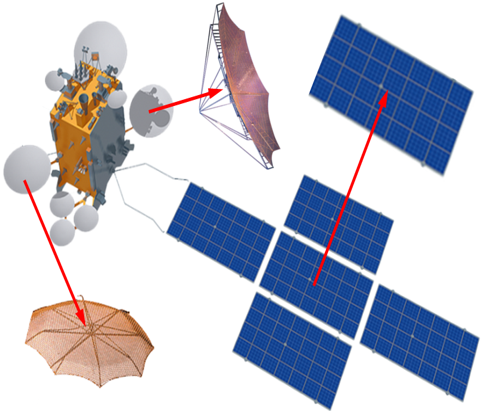
\includegraphics[width = \textwidth]{decomposition}
	\end{subfigure}
	\hfill
	\begin{subfigure}[b]{0.45\textwidth}
	     % Определение стиля
        \tikzstyle{blockWide} = [rectangle, draw = black, fill = blue!15, rounded corners, text width = 20em, text centered, minimum height = 1.5em, drop shadow] 
        \tikzstyle{blockWideC} = [blockWide, fill = red!20]
        \tikzstyle{arrow} = [draw, thick, color = black!90, -latex'] 
        \scriptsize 
        % Задание перменных
        \def\nodeDist{0.3cm}
        % Отрисовка блок-схемы
        \begin{tikzpicture}[scale = 1, transform shape]
            % Задание узлов		
            \node (modalTests) [blockWide] {Модальные испытания \\ составных частей конструкции};
            \node (modelUpdating) [blockWide, below = \nodeDist of modalTests] {Коррекция расчетных моделей \\ составных частей  конструкции \\ по результатам испытаний};
            \node (checkInfluence) [blockWide, below = \nodeDist of modelUpdating] {Освобождение расчетных моделей \\ составных частей конструкции};
            \node (buildRealModel) [blockWide, below = \nodeDist of checkInfluence] {Синтез расчетной модели полной \\ конструкции из её составных частей};
            \node (buildMathModel) [blockWide, below = \nodeDist of buildRealModel] {Определение динамических \\ характеристик полной расчетной модели};
            % Соединение узлов
            \draw [arrow] (modalTests.south) -- (modelUpdating.north);
            \draw [arrow] (modelUpdating.south) -- (checkInfluence.north);
            \draw [arrow] (checkInfluence.south) -- (buildRealModel.north);
            \draw [arrow] (buildRealModel.south) -- (buildMathModel.north);
        \end{tikzpicture}
	\end{subfigure}
    \caption{Схема методики верификации расчетных моделей крупногабаритных трансформируемых конструкций} \label{fig:schemeDecomposition}
    \vspace{1em}
\end{figure}  

Проводится коррекция составных частей тестового космического аппарата: панелей солнечных батарей и орбитального модуля, используя одновременно данные двух виртуальных экспериментов. Затем осуществляется ассемблирование скорректированных моделей. Максимальная погрешность в частотах синтезированной модели до коррекции равнялась $ 5.121 $ \%, а после коррекции составила $ 0.1 $ \%. Распределение изменений узловых жесткостей по всем линейным степеням свободы для моделей составных частей показано на рисунке~\ref{fig:test-spacecraft-distribution}. 

\begin{figure}[!htb]
	\centering
	\begin{subfigure}[t]{0.46\textwidth}
		\centering
		\includegraphics[width = \textwidth]{test-spacecraft-orbital-distribution}
		\caption{Орбитальный модуль} \label{subfig:test-orbital-distribution}
	\end{subfigure}
	\hfill
	\begin{subfigure}[t]{0.44\textwidth}
		\centering
		\includegraphics[height = \textwidth]{test-spacecraft-panel-distribution}
		\caption{Панели солнечных батарей} \label{subfig:test-panel-distribution}
	\end{subfigure}
	\vspace{1em}
	\caption{Распределение изменений узловых жесткостей при коррекции моделей составных частей} \label{fig:test-spacecraft-distribution} 
\end{figure}

\pdfbookmark[1]{Глава 3. Результаты модальных испытаний как исходные данные для коррекции расчетных моделей конструкций}{partModalAnalysis}

\highlight{В третьей главе} развиваются методы классического и операционного модального анализа, позволяющие получать достоверные оценки динамических параметров для коррекции. С целью обеспечения возможности эффективного расчета обобщенных характеристик по результатам модальных испытаний, составлена программная реализация, позволяющая посредством графического интерфейса~\figref{subfig:gencalc-interface} гибко менять параметры расчета и исследовать зависимости получаемых характеристик несколькими способами одновременно. 

Одним из ключевых требований обеспечения непрерывности производственного процесса авиационной техники является сокращение времени между натурными испытаниями и первым вылетом изделия. Поэтому разработана программа~\figref{subfig:analyzer-interface}, использующая программный интерфейс \name{Testlab Automation} для обработки и представления результатов модального анализа непосредственно в процессе испытаний.

\begin{figure}[!htb]
	\centering
	\begin{subfigure}[t]{0.45\textwidth}
		\centering
		\includegraphics[width = \textwidth]{gencalc-interface}
		\caption{Определение модальных параметров} \label{subfig:gencalc-interface}
	\end{subfigure}
	\hfill
	\begin{subfigure}[t]{0.52\textwidth}
		\centering
		\includegraphics[width = \textwidth]{analyzer-interface}
		\caption{Экспресс-представление результатов} \label{subfig:analyzer-interface}
	\end{subfigure}
	\vspace{1em}
	\caption{Программы для обработки и представления результатов модальных испытаний} 
\end{figure}

\noindent
\begin{minipage}{.6\columnwidth}
\hspace{2.5em} Изложена методика контроля зазоров в технических изделиях по искажениям портретов вынужденных колебаний в процессе вибрационных испытаний. Представлен способ поэтапного выявления всех зазоров в объекте испытаний, которые приводят к искажениям портретов колебаний. В рамках описываемого подхода разработана и введена в программное обеспечение управления испытаниями подпрограмма анализа портретов колебаний. Методика обнаружения зазоров по искажениям портретов колебаний использована для диагностирования самолётов в процессе модальных испытаний~\figref{subfig:distortion-high-lift}, а также космических аппаратов открытого исполнения в технологических вибрационных испытаниях~\figref{subfig:distortion-spacecraft}. 
\end{minipage}
\hfill
\begin{minipage}{.4\columnwidth}
	\centering
	\includegraphics[width = 0.75\textwidth]{distortion-high-lift} 
	\captionof{figure}{Зазоры в проводках управления механизацией крыла} \label{subfig:distortion-high-lift}
	\includegraphics[width = 0.6\textwidth]{distortion-spacecraft} 
	\captionof{figure}{Зазоры в узлах установки солнечных батарей} \label{subfig:distortion-spacecraft}
\end{minipage}











